\let\negmedspace\undefined
\let\negthickspace\undefined
\documentclass[journal,12pt,onecolumn]{IEEEtran}
\usepackage{cite}
\usepackage{amsmath,amssymb,amsfonts,amsthm}
\usepackage{algorithmic}
\usepackage{graphicx}
\graphicspath{{./figs/}}
\usepackage{textcomp}
\usepackage{xcolor}
\usepackage{txfonts}
\usepackage{listings}
\usepackage{enumitem}
\usepackage{mathtools}
\usepackage{gensymb}
\usepackage{comment}
\usepackage{caption}
\usepackage[breaklinks=true]{hyperref}
\usepackage{tkz-euclide} 
\usepackage{listings}
\usepackage{gvv}                                        
%\def\inputGnumericTable{}                                 
\usepackage[latin1]{inputenc}     
\usepackage{xparse}
\usepackage{color}                                            
\usepackage{array}                                            
\usepackage{longtable}                                       
\usepackage{calc}                                             
\usepackage{multirow}
\usepackage{multicol}
\usepackage{hhline}                                           
\usepackage{ifthen}                                           
\usepackage{lscape}
\usepackage{tabularx}
\usepackage{array}
\usepackage{float}


\begin{document}
\clearpage
\begin{center}
    \huge{XL: LIFE SCIENCES}\\
    \large{AI25BTECH11001 - Abhisek Mohapatra}\\
    \large{GRADUATE APTITUDE TEST IN ENGINEERING}
\end{center}

\textbf{General Aptitude (GA)}
\textbf{Q.1 -- Q.5 Carry ONE mark Each}

\begin{enumerate}
	\item{ The village was nestled in a green spot,the ocean and the hills.}
    \begin{enumerate}
        \item through
        \item in
        \item at
        \item between
    \end{enumerate}

    \item Disagree : Protest :: Agree : \_\_\_\_\_ (By word meaning)
    \begin{enumerate}
        \item Refuse
        \item Pretext
        \item Recommend
        \item Refute
    \end{enumerate}

    \item A 'frabjous' number is defined as a 3 digit number with all digits odd, and no two adjacent digits being the same. For example, 137 is a frabjous number, while 133 is not. How many such frabjous numbers exist?
    \begin{enumerate}
        \item 125
        \item 720
        \item 60
        \item 80
    \end{enumerate}

    \item Which one among the following statements must be TRUE about the mean and the median of the scores of all candidates appearing for GATE 2023?
    \begin{enumerate}
        \item The median is at least as large as the mean.
        \item The mean is at least as large as the median.
        \item At most half the candidates have a score that is larger than the median.
        \item At most half the candidates have a score that is larger than the mean.
    \end{enumerate}

    \item In the given diagram, ovals are marked at different heights (A) of a hill. Which one of the following options P, Q, R, and S depicts the top view of the hill?
	    \begin{figure}[H]
		\centering
	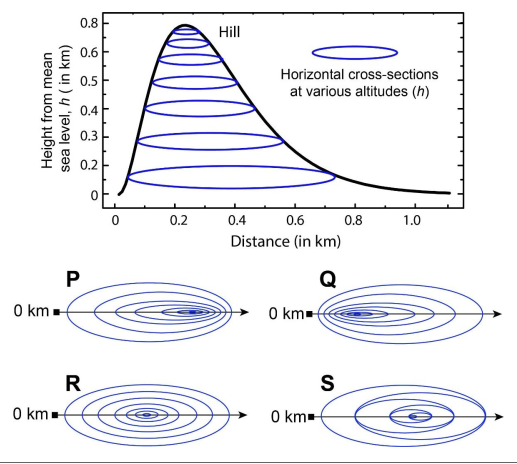
\includegraphics[scale=0.3]{5}
		    \caption*{}
		\label{fig:Q5}
	\end{figure}
    \begin{enumerate}
        \item P
        \item Q
        \item R
        \item S
    \end{enumerate}

\subsection*{Q.6 -- Q.10 Carry TWO marks Each}

    \item Residency is a famous housing complex with many well-established individuals among its residents. A recent survey conducted among the residents of the complex revealed that all of those residents who are well established in their respective fields happen to be academicians. The survey also revealed that most of these academicians are authors of some best-selling books.\\
    Based only on the information provided above, which one of the following statements can be logically inferred with certainty?
    \begin{enumerate}
        \item Some residents of the complex who are well established in their fields are also authors of some best-selling books.
        \item All academicians residing in the complex are well established in their fields.
        \item Some authors of best-selling books are residents of the complex who are well established in their fields.
        \item Some academicians residing in the complex are well established in their fields.
    \end{enumerate}

    \item Ankita has to climb 5 stairs starting at the ground, while respecting the following rules:\\
    1. At any stage, Ankita can move either one or two stairs up.\\
    2. At any stage, Ankita cannot move to a lower step.\\
    Let F(N) denote the number of possible ways in which Ankita can reach the N-th stair. For example, F(1) = 1, F(2) = 2, F(3) = 3.\\
    The value of F(5) is \_\_\_\_\_.
    \begin{enumerate}
        \item 8
        \item 7
        \item 6
        \item 5
    \end{enumerate}

    \item The information contained in DNA is used to synthesize proteins that are necessary for the functioning of life. DNA is composed of four nucleotides: Adenine (A), Thymine (T), Cytosine (C), and Guanine (G). The information contained in DNA can then be thought of as a sequence of these four nucleotides: A, T, C, and G. DNA has coding and non-coding regions. Coding regions---where the sequence of these nucleotides are read in groups of three to produce individual amino acids---constitute only about 2\% of human DNA. For example, the triplet of nucleotides CCG codes for the amino acid glycine, while the triplet GGA codes for the amino acid proline. Multiple amino acids are then assembled to form a protein.
    Based only on the information provided above, which of the following statements can be logically inferred with certainty?
    (i) The majority of human DNA has no role in the synthesis of proteins.
    (ii) The function of about 98\% of human DNA is not understood.
    \begin{enumerate}
        \item only (i)
        \item only (ii)
        \item both (i) and (ii)
        \item neither (i) nor (ii)
    \end{enumerate}

    \item Which one of the given figures P, Q, R and S represents the graph of the following function?
    F(x) = |x + 2| - |x - 1|
    \begin{figure}[H]
		\centering
	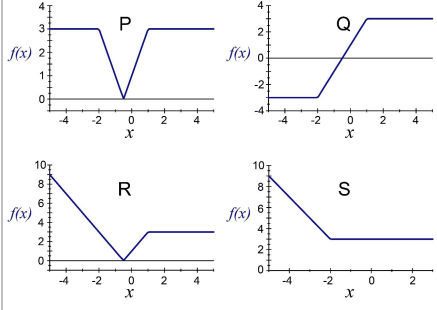
\includegraphics[scale=0.5]{9}
		    \caption*{}
		\label{fig:Q9}
	\end{figure}
    \begin{enumerate}
        \item P
        \item Q
        \item R
        \item S
    \end{enumerate}

    \item An opaque cylinder is suspended in the path of a parallel beam of light, such that its shadow is cast on a screen oriented perpendicular to the direction of the light beam. The cylinder can be reoriented in any direction within the light beam. Under these conditions, which one of the shadows P, Q, R, and S is NOT possible?\\
\begin{figure}[H]
		\centering
	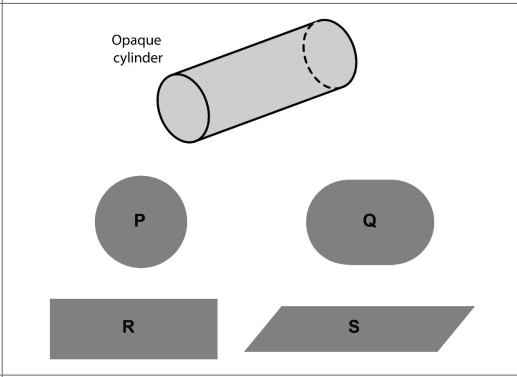
\includegraphics[scale=0.5]{10}
		    \caption*{}
		\label{fig:Q10}
	\end{figure}
    \begin{enumerate}
        \item P
        \item Q
        \item R
        \item S
    \end{enumerate}

\section*{Chemistry --- P (Compulsory)}
\subsection*{XL-P: Q.11 - Q.19 Carry ONE mark Each}

    \item Which one among the following mixtures gives a buffer solution in water?
    \begin{enumerate}
        \item CH3COOH + CH3COONa
        \item CH3COOH + NaCl
        \item NaOH + NaCl
        \item NaOH + CH3COONa
    \end{enumerate}

    \item What is the major product formed in the given reaction?\\
    \begin{figure}[H]
		\centering
	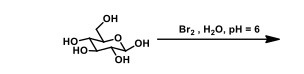
\includegraphics[scale=]{12}
		    \caption*{}
		\label{fig:Q12}
	\end{figure}
    \begin{enumerate}
        \item \begin{figure}[H]
		\centering
            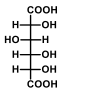
\includegraphics{12a}
		    \caption*{}
		\label{fig:Q12a}
	\end{figure}
        \item \begin{figure}[H]
		\centering
            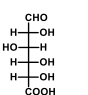
\includegraphics{12b}
		    \caption*{}
		\label{fig:Q12b}
	\end{figure}
        \item \begin{figure}[H]
		\centering
            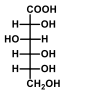
\includegraphics{12c}
		    \caption*{}
		\label{fig:Q12c}
	\end{figure}        
\item \begin{figure}[H]
		\centering
            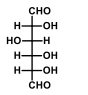
\includegraphics{12d}
		    \caption*{}
		\label{fig:Q12d}
	\end{figure}
    \end{enumerate}

    \item The CORRECT order of stability of the given metal oxides is
    \begin{enumerate}
        \item $LiO2 > NaO2 > KO2 > RbO2$
        \item $LiO2 < NaO2 < KO2 < RbO2$
        \item $LiO2 < NaO2 > KO2 > RbO2$
        \item $LiO2 > NaO2 < KO2 < RbO2$
    \end{enumerate}

    \item Which of the following is/are CORRECT when two single complementary strands of DNA come together to form a double helix at a given temperature? (Delta S and Delta H are changes in entropy and enthalpy of the process, respectively.)
    \begin{enumerate}
        \item $\Delta S > 0$
        \item $\Delta S < 0$
        \item $\Delta H > 0$
        \item $\Delta H < 0$
    \end{enumerate}

    \item Suitable reagent(s) to bring about the conversion of P to Q in good yield is/are
    \begin{figure}[H]
		\centering
	    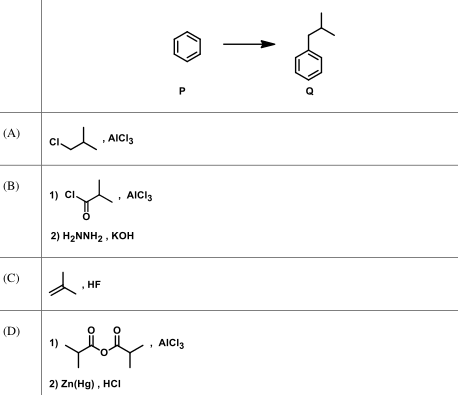
\includegraphics[scale=0.6]{15}
		    \caption*{}
		\label{fig:Q15}
	\end{figure}

    \item Choose the CORRECT trend(s) of the first ionization energies among the following. (Given: Atomic numbers C: 6; N: 7; O: 8; F: 9; Si: 14; P: 15; S: 16; Cl: 17)
    \begin{enumerate}
        \item $C < N > O < F$
        \item $Si < P > S < Cl$
        \item $C < N < O < F$
        \item $Si < P < S < Cl$
    \end{enumerate}

    \item The depression of freezing point of water (in K) for 0.1 molal solutions of NaCl and Na2SO4 are Delta T1 and Delta T2, respectively. Assuming the solutions to be ideal, the ratio Delta T1 / Delta T2 is (rounded off to two decimal places).

    \item Considering cyclobutane to be planar, the number of planes of symmetry in the following compound is (in integer).\\
    \begin{figure}[H]
		\centering
            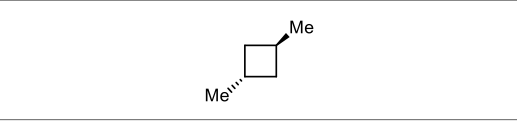
\includegraphics{18}
		    \caption*{}
		\label{fig:Q18}
	\end{figure}


    \item The dipole moment (mu) of BrF is 1.42 D and the bond length is 176 pm. The atomic charge distribution (q) in the molecule is (rounded off to two decimal places). (Given: 1 D = 3.34 x 10$^{-30}$ C m; the factor e (electronic charge) = 1.60 x 10$^{-19}$ C)

\subsection*{XL-P: Q.20 --- Q.27 Carry TWO marks Each}

    \item Consider two different paths in which the volume of an ideal gas doubles isothermally:\\
    i) Reversible expansion (work done = Wrev)\\
    ii) Irreversible expansion, with the external pressure equal to the final pressure of the gas (work done = Wirrev)\\
    Here, Wrev / Wirrev
    \begin{enumerate}
        \item 2 ln 2
        \item 1 / (2 ln 2)
        \item 3 ln 2
        \item 1 / (3 ln 2)
    \end{enumerate}

    \item A mixture of four peptides, PRKRK, RGERV, RYRGV, and LVVYP, is loaded onto an ion-exchange column at pH = 7.2. If carboxymethyl (CM) cellulose is used as the stationary phase of this column, then which peptide elutes first?\\
    (Given: Cellulose - CM-cellulose, Amino acids info)
    \begin{figure}[H]
		\centering
            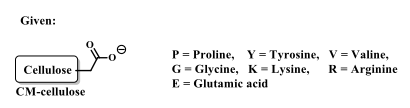
\includegraphics{21}
		    \caption*{}
		\label{fig:Q21}
	\end{figure}

     Choose the CORRECT trend(s) of the first ionization energies among the following. (Given: Atomic numbers C: 6; N: 7; O: 8; F: 9; Si: 14; P: 15; S: 16; Cl: 17)
    \begin{enumerate}
        \item PRKRK
        \item RGERV
        \item RYRGV
        \item LVVYP
    \end{enumerate}

    \item Match the coordination complexes given in Group I with the most appropriate properties in Group II. (Given: Atomic numbers of Mn: 25; Co: 27; Ni: 28)
    

    \begin{minipage}{0.45\textwidth}
	    \begin{enumerate}
        \item[P.] [Mn(H$_2$O)6]$^2+$
        \item[Q.] [CoF6]$^{3-}$
        \item[R.] [NiCl4]$^{2-}$
        \item[S.] [Ni(CN)4]$^{2-}$
    \end{enumerate}
    \end{minipage}
    \begin{minipage}{0.45\textwidth}
    \begin{enumerate}
        \item 5.92 Bohr Magneton (BM)
        \item CFSE=0.4$\Delta_o$
        \item Metal ion hybridisation is sp$^3$
        \item Diamagnetic
    \end{enumerate}
    \end{minipage}
    \begin{enumerate}
        \item E-1, F-2, G-3, H-4
        \item E-2, F-1, G-4, H-3
        \item E-4, F-2, G-1, H-3
        \item E-1, F-4, G-3, H-2
    \end{enumerate}

    \item Compounds P and Q undergo E2 elimination with reaction rate constants of kP and kQ, respectively, as shown below. Which is/are the CORRECT option(s)?\\
    
    \begin{figure}[H]
		\centering
	    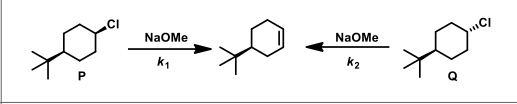
\includegraphics[scale=0.5]{23}
		    \caption*{}
		\label{fig:Q23}
	\end{figure}

     Choose the CORRECT trend(s) of the first ionization energies among the following. (Given: Atomic numbers C: 6; N: 7; O: 8; F: 9; Si: 14; P: 15; S: 16; Cl: 17)

    \begin{enumerate}
        \item $kP > kQ$
        \item $kQ > kP$
        \item Most stable conformer of P gives the product
        \item Most stable conformer of Q gives the product
    \end{enumerate}

    \item According to Hard-Soft Acid-Base (HSAB) principle, the CORRECT option(s) for the solubility trend in water is/are
    \begin{enumerate}
        \item $AgF > AgCl > AgBr > AgI$
        \item $LiBr > LiCl > LiF$
        \item $AgF < AgCl < AgBr < AgI$
        \item $LiBr < LiCl < LiF$
    \end{enumerate}

    \item Compound X gives alcohol P as the major product for the reaction shown below. Suitable option(s) for X is/are\\
    \begin{figure}[H]
		\centering
	    
\includegraphics[scale=0.5]{25}
		    \caption*{}
		\label{fig:Q25}
	\end{figure}
    \begin{enumerate}
        \item \begin{figure}[H]
		\centering
            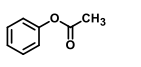
\includegraphics{25a}
		    \caption*{}
		\label{fig:Q25a}
	\end{figure}
        \item \begin{figure}[H]
		\centering
            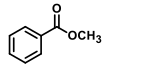
\includegraphics{25b}
		    \caption*{}
		\label{fig:Q25b}
	\end{figure}
        \item \begin{figure}[H]
		\centering
            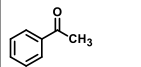
\includegraphics{25c}
		    \caption*{}
		\label{fig:Q25c}
	\end{figure}
        \item \begin{figure}[H]
		\centering
            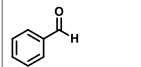
\includegraphics{25d}
		    \caption*{}
		\label{fig:Q25d}
	\end{figure}
    \end{enumerate}

    \item The number of radial node(s) for the valence orbital of UCl$_6^-$ ion is (in integer). (Given: Atomic number of U is 92)

    \item E$^o$ = 1.10 V for the following cell reaction: Zn(s) + Cu$^2+$(aq) $\leftrightarrow$ Zn$^2+$(aq) + Cu(s)\\
    For this reaction, the equilibrium constant is y x 10$^{37}$ at 298 K. The value of y is (rounded off to two decimal places). (Given: F = 96485 C mol$^-1$, R=8.314 J K$^-1$ mol$^-1$)

\section*{Biochemistry (XL-Q)}
\subsection*{XL-Q: Q.28 --- Q.35 Carry ONE mark Each}

    \item Determine the correctness or otherwise of the following Assertion [a] and the Reason [r].\\
    Assertion [a]: On a per carbon basis, palmitic acid yields more ATP than glucose.\\
    Reason [r]: Carbons in palmitic acid are more reduced than those in glucose.
    \begin{enumerate}
        \item Both [a] and [r] are true and [r] is the correct reason for [a]
        \item Both [a] and [r] are true but [r] is not the correct reason for [a]
        \item [a] is true but [r] is false
        \item [a] is false but [r] is true
    \end{enumerate}

    \item When cell components are fractionated by sedimentation, the correct order (from lower to higher gravitational force, g) in which the components get separated is
    \begin{enumerate}
        \item nuclei, mitochondria, microsomes, and ribosomes
        \item microsomes, mitochondria, ribosomes, and nuclei
        \item nuclei, ribosomes, mitochondria, and microsomes
        \item ribosomes, microsomes, mitochondria, and nuclei
    \end{enumerate}

    \item In a population, the probability of a susceptible individual getting infected with SARS-CoV-2 is low when a majority of individuals in the population becomes immune to this virus. This phenomenon is known as
    \begin{enumerate}
        \item innate immunity
        \item adaptive immunity
        \item active immunity
        \item herd immunity
    \end{enumerate}

    \item Given below are four reactions of the glycolytic pathway catalyzed by the enzymes E1, E2, E3, and E4, as indicated. Which of these enzymes is/are NOT part of the gluconeogenesis pathway?
    
    (i) Fructose 6-phosphate -> Fructose 1,6-bisphosphate (E1)
    
    (ii) Fructose 1,6-bisphosphate -> Dihydroxyacetone phosphate + Glyceraldehyde 3-phosphate (E2)
    
    (iii) 3-Phosphoglycerate -> 2-Phosphoglycerate (E3)
    
    (iv) Phosphoenolpyruvate -> Pyruvate (E4)
    \begin{enumerate}
        \item E1
        \item E2
        \item E3
        \item E4
    \end{enumerate}

    \item Which of the following molecules is/are second messenger(s) produced by the phosphoinositide signaling cascade?
    \begin{enumerate}
        \item Phosphatidylinositol 4,5-bisphosphate
        \item Inositol 1,4,5-triphosphate
        \item Inositol 1,3,5-triphosphate
        \item Diacylglycerol
    \end{enumerate}

    \item A protein has seven cysteine residues. The maximum number of disulfide bonds of different combinations that can possibly be formed by these seven cysteine residues is (in integer).

    \item A lyophilized sample of 20 nanomoles of an oligonucleotide is dissolved in water and the volume of the solution is made up to 200 microL. The concentration (in microM) of the oligonucleotide in this solution is (in integer).

    \item DNA in a 1 cm long chromatin contains 5 x 10$^9$ base pairs. The fold compaction of this DNA within the chromatin is (in integer).

\subsection*{XL-Q: Q.36 --- Q.46 Carry TWO marks Each}

    \item Intracellular concentrations of ATP, ADP, and inorganic phosphate in four cell types are given below. Which one of these cell types has the most negative Delta G for ATP hydrolysis?\\
    \begin{tabular}{lccc}
    Cell type & ATP (mM) & ADP (mM) & Inorganic phosphate (mM) \\
    L & 3.0 & 1.8 & 5.0 \\
    K & 3.9 & 1.3 & 3.0 \\
    B & 2.7 & 0.7 & 2.7 \\
    M & 7.2 & 0.9 & 8.0 \\
    \end{tabular}
    \begin{enumerate}
        \item L
        \item K
        \item B
        \item M
    \end{enumerate}

    \item Which one of the following amino acids has more than two acid-base groups?
    \begin{enumerate}
        \item Alanine
        \item Leucine
        \item Phenylalanine
        \item Tyrosine
    \end{enumerate}

    \item Enzyme activity profiles as a function of time in the absence or presence of different types of feedback mechanisms are shown in the figure below. Match the following feedback mechanisms with the corresponding profiles in the figure.
        [p.] No feedback mechanism
        [q.] Negative feedback mechanism with short delay
        [r.] Negative feedback mechanism with long delay
        [s.] Positive feedback mechanism
\begin{figure}[H]
		\centering
            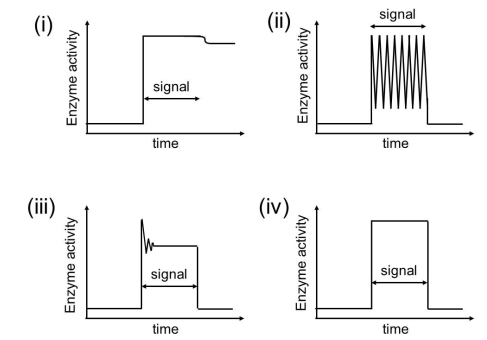
\includegraphics{38}
		    \caption*{}
		\label{fig:Q38}
	\end{figure}
    \begin{enumerate}
        \item (p)-(i); (q)-(ii); (r)-(iii); (s)-(iv)
        \item (p)-(iv); (q)-(i); (r)-(ii); (s)-(iii)
        \item (p)-(iv); (q)-(ii); (r)-(i); (s)-(iii)
        \item (p)-(iii); (q)-(ii); (r)-(i); (s)-(iv)
    \end{enumerate}

    \item A linear DNA fragment of 5 kilobase (kb) when completely digested with EcoRI produces 2.5 kb, 1.5 kb, and 1 kb fragments. Complete digestion of the same 5 kb fragment with XbaI produces 3.5 kb and 1.5 kb fragments. Which one of the following sets of fragments will be obtained if the 5 kb fragment is fully digested with EcoRI and XbaI simultaneously?
    \begin{enumerate}
        \item 3 kb and 2 kb
        \item 2 kb and 1 kb
        \item 2 kb, 1.5 kb, 1 kb, and 0.5 kb
        \item 2.5 kb, 1.5 kb, 0.75 kb, and 0.25 kb
    \end{enumerate}

    \item \begin{minipage}{0.45\textwidth}
    Match the cell types listed in Group I with associated processes listed in Group II.
    \begin{itemize}
        \item[p.] NK cells
        \item[q.] B cells
        \item[r.] Mast cells
        \item[s.] Neutrophils
    \end{itemize}
    \end{minipage}
    \begin{minipage}{0.45\textwidth}
    \begin{itemize}
        \item[i.] Antibody production
        \item[ii.] First cells to be recruited at the site of infection
        \item[iii.] Antibody-dependent cell-mediated cytotoxicity
        \item[iv.] Histamine production
    \end{itemize}
    \end{minipage}
    \begin{enumerate}
        \item (p)-(iii); (q)-(i); (r)-(iv); (s)-(ii)
        \item (p)-(iii); (q)-(i); (r)-(iv); (s)-(ii)
        \item (p)-(iii); (q)-(i); (r)-(iv); (s)-(ii)
        \item (p)-(iii); (q)-(i); (r)-(ii); (s)-(iv)
    \end{enumerate}

    \item Four statements about lipids are given below as options. Choose the statement(s) which is/are CORRECT.
    \begin{enumerate}
        \item Cholesterol is amphipathic
        \item Self-assembly of phospholipids in water is due to hydrophobic effect
        \item The temperature at which the gel phase changes to liquid crystalline phase increases with an increase in the degree of unsaturation of fatty acyl tails
        \item The choline head group of lipids is positively charged
    \end{enumerate}

    \item Which of the following technique(s) can be used to separate proteins according to their molecular weights from a mixture of proteins?
    \begin{enumerate}
        \item Ion exchange chromatography
        \item Size exclusion chromatography
        \item Sodium dodecylsulfate --- polyacrylamide gel electrophoresis (SDS-PAGE)
        \item Sucrose density gradient centrifugation
    \end{enumerate}

    \item B cells produce two forms of an immunoglobulin: (i) membrane-bound form, known as B cell receptor (BCR) and (ii) soluble form, known as antibody. Which of the following statements is/are CORRECT about BCR and antibody produced by the same B cell?
    \begin{enumerate}
        \item BCR and antibody have identical antigen binding site
        \item BCR and antibody recognize different epitopes
        \item BCR and antibody are encoded by the same gene
        \item BCR and antibody are formed by differential splicing
    \end{enumerate}

    \item A 100 ml solution of pH 10 was well-mixed with a 100 ml solution of pH 4. The pH of the resultant 200 ml solution is rule{1 cm}{0.15 mm} (rounded off to two decimal places).

    \item An organism uses only the glycerophosphate shunt pathway to transport cytosolic NADH to mitochondria. For every two electrons transported, complex I, complex III, and complex IV of the electron transport chain in this organism transport 2.5, 1.5, and 2.0 protons (H$^+$), respectively. The H$^+$ to ATP ratio of F0F1-ATPase of this organism is 4.0. Terminal electron acceptor is oxygen.
    The number of ATP molecules synthesized by oxidizing NADH from glycolysis is \rule{1 cm}{0.15 mm} (rounded off to two decimal places).

    \item If the extracellular concentration of sodium ion (Na$^+$) is ten times more than its intracellular concentration, then the sodium equilibrium potential at 20 $\degree$C in mV is \rule{1 cm}{0.15 mm} (rounded off to two decimal places). Assume that the membrane is permeable only to Na$^+$ ions. (Use R = 1.987 cal deg$^-1$ mol$^-1$ and F = 23062 cal mol$^-1$ V$^-1$)

\section*{Botany (XL-R)}
\subsection*{XL-R: Q.47 --- Q.54 Carry ONE mark Each}

    \item Which one of the following statements on Casparian strips is correct?
    \begin{enumerate}
        \item Casparian strips are specific to vascular plants found in epidermal cells.
        \item Casparian strips are modifications mostly found in shoot tissue.
        \item Casparian strips act as a cellular barrier to allow selective nutrient uptake and exclusion of pathogens.
        \item Casparian strips are common in root endodermal cells of non-vascular plants.
    \end{enumerate}

    \item Rotenone is a chemical often used to kill insect pests on crop plants and fishes in lakes. Rotenone acts by inhibiting electron transport from the NADH dehydrogenase enzyme in Complex I to ubiquinone in the mitochondrial electron transport chain. Which one of the following explains why plants can tolerate rotenone application?
    \begin{enumerate}
        \item The Complex I in plants is resistant to rotenone.
        \item Plants inactivate rotenone by enzymatic degradation.
        \item Plants have specific channels that efflux rotenone out of the cell.
        \item Plants have additional NAD(P)H dehydrogenases that are resistant to rotenone.
    \end{enumerate}

    \item Although Pseudomonas syringae infection in plants is actively inhibited by the endogenous salicylic acid (SA) of host origin, a successful infection is still established because the bacterium secretes coronatine, an effector molecule. Which one of the following best describes the mode of action of coronatine?
    \begin{enumerate}
        \item Coronatine inhibits SA biosynthesis.
        \item Coronatine promotes the biosynthesis of jasmonic acid (JA), and JA signaling in turn inhibits SA response.
        \item Coronatine is a structural analogue of SA, which binds to the SA receptor and inhibits its function.
        \item Coronatine is a structural analogue of jasmonic acid (JA), which activates JA signaling to inhibit SA response.
    \end{enumerate}

    \item The schematic depicts an unexpanded plant cell within a hypocotyl with the arrangement of cellulose microfibrils marked on its cell wall. Which one of the following shapes would most likely result from the expansion of this cell if the pattern of the cellulose fibrils does not change?\\
   \begin{figure}[H]
		\centering
            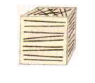
\includegraphics{50}
		    \caption*{}
		\label{fig:Q50}
	\end{figure} 
    \begin{enumerate}
        \item Shape A
   \begin{figure}[H]
		\centering
            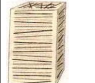
\includegraphics{50a}
		    \caption*{}
		\label{fig:Q50a}
	\end{figure} 
        \item Shape B
   \begin{figure}[H]
		\centering
            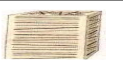
\includegraphics{50b}
		    \caption*{}
		\label{fig:Q50b}
	\end{figure} 
        \item Shape C
   \begin{figure}[H]
		\centering
            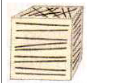
\includegraphics{50c}
		    \caption*{}
		\label{fig:Q50c}
	\end{figure} 
        \item Shape D
   \begin{figure}[H]
		\centering
            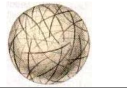
\includegraphics{50d}
		    \caption*{}
		\label{fig:Q50d}
	\end{figure} 
    \end{enumerate}

    \item Which one or more of the following statements is/are NOT CORRECT with respect to pollen development in angiosperm?
    \begin{enumerate}
        \item Tapetal cell wall in all angiosperms breaks down to release the cytoplasmic content.
        \item Tapetal cell wall in all angiosperms remains intact.
        \item Tapetal cell wall breaks down in some angiosperm species, whereas it remains intact in others.
        \item Within an angiosperm species, the tapetal cell wall breaks down in some individuals and not in others.
    \end{enumerate}

    \item Regulation of phosphoenolpyruvate carboxylase (PEPCase) governs CO2 fixation in both C4 and CAM (crassulacean acid metabolism) plants. Which one or more of the following statements with respect to PEPCase activity is/are CORRECT?
    \begin{enumerate}
        \item PEPCase in C4 plants is inactivated by dephosphorylation during the day.
        \item PEPCase in CAM plants is inactivated by dephosphorylation during the day.
        \item PEPCase in C4 plants is inactivated by dephosphorylation at night.
        \item PEPCase in CAM plants is inactivated by dephosphorylation at night.
    \end{enumerate}

    \item Which one or more processes listed below DOES NOT/DO NOT produce carbon dioxide during fermentation?
    \begin{enumerate}
        \item Brewing wine using yeast.
        \item Baking bread using yeast.
        \item Making yogurt using lactobacillus.
        \item Making cheese using fungus.
    \end{enumerate}

    \item The ovule of a diploid species with 2n = 8 undergoes double fertilization. If the pollen is contributed by an individual with meiotic nondisjunction, the chromosome number of the zygote will be \rule{1 cm}{0.15 mm}.

\subsection*{XL-R: Q.55 --- Q.65 Carry TWO marks Each}

    \item \begin{minipage}{0.45\textwidth}
    Match the tasks given in Group I with the associated techniques conventionally used as listed in Group II.
    \begin{itemize}
        \item[P.] Ploidy analysis
        \item[Q.] Profiling DNA methylation
        \item[R.] Identifying non-coding RNAs
        \item[S.] Identifying SNPs
        \item[T.] Satellite DNA isolation
    \end{itemize}
    \end{minipage}
    \begin{minipage}{0.45\textwidth}
    \begin{itemize}
        \item[1.] RNA sequencing
        \item[2.] Exome sequencing
        \item[3.] Fluorescence in situ hybridization
        \item[4.] Bisulfite sequencing
        \item[5.] Density-gradient centrifugation
    \end{itemize}
    \end{minipage}
    \begin{enumerate}
        \item P-2; Q-1; R-3; S-4; T-5
        \item P-3; Q-4; R-1; S-2; T-5
        \item P-5; Q-4; R-1; S-2; T-3
        \item P-3; Q-5; R-1; S-2; T-4
    \end{enumerate}

    \item \begin{minipage}{0.45\textwidth}
    Periderm is a protective tissue found in stems and roots of gymnosperm and woody dicotyledons. It contributes to the increased thickness by secondary growth. Match the peridermal components given in Group I with the cell/tissue types given in Group II.
    \begin{itemize}
        \item[P.] Phelloids
        \item[Q.] Phellogen
        \item[R.] Phellem
        \item[S.] Phelloderm
    \end{itemize}
    \end{minipage}
    \begin{minipage}{0.45\textwidth}
    \begin{itemize}
        \item[1.] Tissue resembling cortical parenchyma
        \item[2.] Cork cambium
        \item[3.] Cork-like cells
        \item[4.] Cork
    \end{itemize}
    \end{minipage}
    \begin{enumerate}
        \item P-4; Q-3; R-1; S-2
        \item P-3; Q-2; R-4; S-1
        \item P-2; Q-1; R-3; S-4
        \item P-4; Q-1; R-3; S-2
    \end{enumerate}

    \item \begin{minipage}{0.45\textwidth}
    Match the following rice diseases in Group I with their causal agents in Group II.
    \begin{itemize}
        \item[P.] Blast
        \item[Q.] False smut
        \item[R.] Sheath blight
        \item[S.] Downy mildew
    \end{itemize}
    \end{minipage}
    \begin{minipage}{0.45\textwidth}
    \begin{itemize}
        \item[1.] Sclerophthora macrospora
        \item[2.] Rhizoctonia solani
        \item[3.] Ustilaginoidea virens
        \item[4.] Puccinia graminis
        \item[5.] Magnaporthe grisea
    \end{itemize}
    \end{minipage}
    \begin{enumerate}
        \item P-5; Q-3; R-2; S-1
        \item P-4; Q-2; R-5; S-3
        \item P-4; Q-5; R-3; S-1
        \item P-5; Q-4; R-1; S-2
    \end{enumerate}

    \item 
    Central vascular cylinder or stele consists of the primary vascular system (xylem and phloem) and the associate fundamental tissue. Match the schematics of stele in Group I (xylem shown in green, and phloem shown as A) with their respective types in Group II.
   \begin{figure}[H]
		\centering
             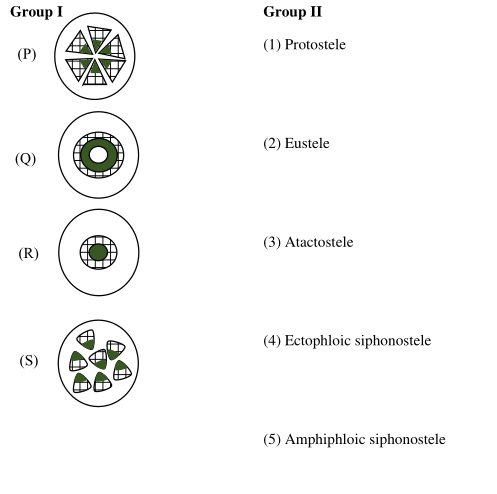
\includegraphics{58}
		    \caption*{}
		\label{fig:Q58}
	\end{figure} 
    \begin{enumerate}
        \item P-2; Q-4; R-1; S-3
        \item P-5; Q-1; R-4; S-2
        \item P-5; Q-3; R-1; S-2
        \item P-3; Q-4; R-2; S-5
    \end{enumerate}

    \item Consider the following four experimental observations (i, ii, iii, iv) on the effect of the FT gene on flowering transition in the shoot apical meristem (SAM) of Arabidopsis thaliana.\\
    i) The FT promoter is active in leaves alone.\\
    ii) The ft null mutation causes delayed flowering transition of the SAM.\\
    iii) Expressing a recombinant FT protein fused to nuclear localization signal sequence under the endogenous promoter does not rescue the delayed-flowering phenotype of the ft null mutant.\\
    iv) Downregulation of FT transcript in the SAM by RNA interference in the wild-type background does not alter flowering transition.\\
    Which one of the following conclusions best explains the above observations?
    \begin{enumerate}
        \item FT protein resident in leaves causes flowering transition of the SAM.
        \item FT transcript moves from leaves to the meristem and promotes flowering.
        \item FT protein moves from leaves to the SAM and promotes flowering.
        \item Both FT transcript and FT protein are required in the SAM to promote flowering.
    \end{enumerate}

    \item \begin{minipage}{0.45\textwidth}
    Which one of the options given correctly matches the alkaloids in Group I with their source plants in Group II?
    \begin{itemize}
        \item[P.] Cocaine
        \item[Q.] Caffeine
        \item[R.] Morphine
        \item[S.] Atropine
    \end{itemize}
    \end{minipage}
    \begin{minipage}{0.45\textwidth}
    \begin{itemize}
        \item[1.] Cocoa
        \item[2.] Nightshade
        \item[3.] Coca
        \item[4.] Poppy
    \end{itemize}
    \end{minipage}
    \begin{enumerate}
        \item P-3; Q-1; R-4; S-2
        \item P-1; Q-3; R-4; S-2
        \item P-2; Q-1; R-3; S-4
        \item P-4; Q-2; R-1; S-3
    \end{enumerate}

    \item A drought tolerant rice genotype was found to be associated with a missense mutation in the gene A. Which one or more of the following experiments is/are appropriate to validate whether the mutation in A is the causal factor for drought tolerance?
    \begin{enumerate}
        \item Introduce the same mutation in a drought sensitive rice genotype and test if it becomes drought tolerant.
        \item Delete the wild-type A in drought sensitive plant and test if it becomes drought tolerant.
        \item Determine the stability of the protein encoded by the wild-type and the mutant forms of A.
        \item Repair the mutation in the drought tolerant rice genotype and test if it becomes drought sensitive.
    \end{enumerate}

    \item Blue light can directly induce opening of stomata. Blue light also triggers photosynthesis in the guard cells, which indirectly induces stomatal opening. Which one or more of the following experimental approaches would test the direct effect of blue light on stomatal opening?
    \begin{enumerate}
        \item Application of low photon fluxes of red light followed by high fluence rate of blue light.
        \item Application of high fluence rates of red light followed by low photon fluxes of blue light.
        \item Application of high fluence rates of blue light followed by high photon fluxes of red light.
        \item Inhibition of photosynthetic electron transport by dichlorophenyldimethylurea (DCMU).
    \end{enumerate}

    \item In a diploid angiosperm species, flower colour is regulated by the R gene. RR and Rr genotypes produce red flowers, whereas the rr genotype produces white flowers. If two individual plants are randomly selected from a large segregating population of a genetic cross between RR and rr parents, the probability of both the plants producing red flowers is \rule{1 cm}{0.15 mm} (Rounded off to two decimal places)

    \item A cytoplasmic male-sterile female plant with the restorer (nuclear) genotype rr is crossed to a male-fertile male plant with the genotype RR. Both RR and Rr can restore the fertility, whereas rr cannot. When an F1 female plant with Rr genotype was test-crossed to a male-fertile male plant with the rr genotype, the percentage of the population that is male fertile would be \rule{1 cm}{0.15 mm} %. (Answer in integer)

    \item The frequencies for autosomal alleles A and a are p = 0.5 and q = 0.5, respectively, where A is dominant over a. Under the assumption of random mating, the mating frequency among dominant parents is \rule{1 cm}{0.15 mm} (Rounded off to two decimal places)

\section*{Microbiology (XL-S)}
\subsection*{XL-S: Q.66 --- Q.73 Carry ONE mark each}

    \item Monkey pox is caused by a
    \begin{enumerate}
        \item double-stranded DNA virus
        \item single-stranded DNA virus
        \item double-stranded RNA virus
        \item single-stranded RNA virus
    \end{enumerate}

    \item Which one of the following converts sulfate to hydrogen sulfide?
    \begin{enumerate}
        \item Beggiatoa
        \item Desulfovibrio
        \item Thiobacillus
        \item Thiothrix
    \end{enumerate}

    \item Which one of the statements about bacterial flagella is correct?
    \begin{enumerate}
        \item Flagella varies in length ranging from 0.5 to 2 micro m.
        \item Flagella are adjacent fibrils with regular patterns.
        \item Flagella helps in conjugation.
        \item Flagella originates from basal body.
    \end{enumerate}

    \item Microbial plastics are made from
    \begin{enumerate}
        \item polyhydroxyalkanoates
        \item polystyrene
        \item polyurethane
        \item polyvinyl chloride
    \end{enumerate}

    \item The correct sequence of metabolic intermediates in Krebs cycle is
    \begin{enumerate}
        \item alpha-ketoglutarate --- fumarate --- succinate --- malate
        \item fumarate --- malate --- succinate --- alpha-ketoglutarate
        \item alpha-ketoglutarate --- succinate --- fumarate --- malate
        \item succinate --- alpha-ketoglutarate --- malate --- fumarate
    \end{enumerate}

    \item Catabolite repression in bacteria is regulated by the concentration of
    \begin{enumerate}
        \item amino acids
        \item glucose
        \item messenger RNA
        \item lactose
    \end{enumerate}

    \item Phagocytosis was first described by
    \begin{enumerate}
        \item Elie Metchnikoff
        \item Robert Hooke
        \item Robert Koch
        \item Paul Ehrlich
    \end{enumerate}

    \item Which one of the following statements about batch culture of microbes is NOT correct?
    \begin{enumerate}
        \item Cells from stationary phase will show longer lag phase when inoculated in fresh growth medium compared to those collected from exponential phase.
        \item Death phase of culture is often exponential in nature.
        \item Stationary phase is the cryptic growth phase.
        \item The rate of generation of new cells during exponential growth phase is constant.
    \end{enumerate}

\subsection*{XL-S: Q.74 --- Q.84 Carry TWO marks each}

    \item \begin{minipage}{0.45\textwidth}
    Match the test in Group I with its application in Group II
    \begin{itemize}
        \item[P.] Oakley-Fulthorpe test
        \item[Q.] Limulus amoebocyte lysate test
        \item[R.] Weil-Felix reaction test
        \item[S.] Complement-fixation test
    \end{itemize}
    \end{minipage}
    \begin{minipage}{0.45\textwidth}
    \begin{itemize}
        \item[1.] IgM detection
        \item[2.] Determining antigen-antibody specificity
        \item[3.] Endotoxin detection
        \item[4.] Rickettsial infection diagnosis
    \end{itemize}
    \end{minipage}
    \begin{enumerate}
        \item P-2, Q-3, R-4, S-1
        \item P-2, Q-1, R-4, S-3
        \item P-3, Q-1, R-2, S-4
        \item P-4, Q-3, R-2, S-1
    \end{enumerate}

    \item Which one of the following is NOT correct about antibiotic resistance mechanism in microbes?
    \begin{enumerate}
        \item Mycoplasma is naturally resistant to penicillins due to presence of R plasmid.
        \item Gram-negative bacteria are impermeable to penicillin G.
        \item beta-lactamases of bacteria can cleave penicillins.
        \item Selective microbes can efflux penicillins entering the cell and develop resistance.
    \end{enumerate}

    \item A suspension of photosynthetic green algae was illuminated in the presence of C$^14O2$ for few seconds. The first metabolite in the Calvin cycle to be radiolabeled will be
    \begin{enumerate}
        \item glyceraldehyde
        \item 1,3-bisphosphoglycerate
        \item 3-phosphoglycerate
        \item ribulose 1,5-bisphosphate
    \end{enumerate}

    \item Determine the correctness or otherwise of the following Assertion [a] and the Reason [r].\\
    Assertion [a]: Endospore can survive heat that would rapidly kill vegetative cells of the same species.\\
    Reason [r]: In endospore, the protoplasm is reduced to minimum volume as a result of the accumulation of calcium-dipicolinic acid complexes and small acid-soluble spore proteins, which forms a cytoplasmic gel and a thick cortex.
    \begin{enumerate}
        \item Both [a] and [r] are true and [r] is the correct reason for [a]
        \item Both [a] and [r] are true and [r] is not the correct reason for [a]
        \item Both [a] and [r] are false
        \item [a] is true but [r] is false
    \end{enumerate}

    \item Which one of the following conjugations will result in formation of merodiploids?
    \begin{enumerate}
        \item F$^+$ donor x F$^-$ recipient
        \item Hfr donor x F$^-$ recipient
        \item F' donor x F$^-$ recipient
        \item F$^+$ donor x Hfr recipient
    \end{enumerate}

    \item Which of the following genus is/are a spirochete(s)?
    \begin{enumerate}
        \item Borrelia
        \item Leptospira
        \item Spirulina
        \item Treponema
    \end{enumerate}

    \item Which of the following is/are non-membrane bound inclusion bodies?
    \begin{enumerate}
        \item Carboxysomes
        \item Cyanophycin granules
        \item Poly-beta-hydroxybutyrate granules
        \item Polyphosphate granules
    \end{enumerate}

    \item Which of the following antibiotics is/are isolated from Streptomyces spp.?
    \begin{enumerate}
        \item Gentamicin
        \item Nystatin
        \item Polymyxins
        \item Tetracyclines
    \end{enumerate}

    \item Which of the following statements about the primary and secondary adaptive immune responses to an antigen is/are correct?
    \begin{enumerate}
        \item IgM antibodies appear first in response to the initial exposure of the antigen.
        \item Majority of the antibodies produced in response to the second exposure of the same antigen are IgM isotype.
        \item Second exposure of the same antigen stimulates production of memory cells.
        \item Primary antibody response has shorter lag phase than secondary antibody response.
    \end{enumerate}

    \item The spontaneous, and induced mutations in bacteria can be distinguished by
    \begin{enumerate}
        \item fluctuation test
        \item replica plating
        \item disc diffusion test
        \item use-dilution test
    \end{enumerate}

    \item During the exponential growth, it took 6 hours for the population of bacterial cells to increase from 2.5 x 10$^6$ to 5 x 10$^7$. The generation time of the bacterium, rounded off to the nearest integer, is \rule{1 cm}{0.15 mm} minutes.

\section*{Zoology (XL-T)}
\subsection*{XL-T: Q.85 --- Q.92 Carry ONE mark Each}

    \item Which one of the following animals has "Book Lungs" as a respiratory organ?
    \begin{enumerate}
        \item Earthworm
        \item Scorpion
        \item Octopus
        \item Starfish
    \end{enumerate}

    \item Which one of the following describes the "innate behavior" of an animal?
    \begin{enumerate}
        \item A behavior that is triggered due to the change in environment.
        \item A behavior that is trained by the parents.
        \item A behavior that is determined by heredity.
        \item A behavior that is learnt by "hit and trial" approach.
    \end{enumerate}

    \item Which one of the following represents a true "Ecological population"?
    \begin{enumerate}
        \item A pitcher plant and a trapped fly in it
        \item All animals that live near each other in a national park
        \item The leeches and the flatworms that live in a forest
        \item All the lions in a reserve forest
    \end{enumerate}

    \item Which of the following animals show "Bottle cells" during the gastrulation stage of development?
    \begin{enumerate}
        \item Snails
        \item Amphibians
        \item Birds
        \item Mammals
    \end{enumerate}

    \item The organisms that obtain energy from inorganic compounds are known as
    \begin{enumerate}
        \item Autotrophs
        \item Organotrophs
        \item Lithotrophs
        \item Phototrophs
    \end{enumerate}

    \item Which of the following is/are the causative agent(s) of Filariasis?
    \begin{enumerate}
        \item Wuchereria bancrofti
        \item Leishmania donovani
        \item Brugia malayi
        \item Trypanosoma gambiense
    \end{enumerate}

    \item In a population of 1000 wild dogs in a grassland, 360 and 480 dogs had black body colour with genotypes BB and Bb, respectively. In the same population, remaining dogs were white in colour with a genotype of bb. Based on this data, the frequency of allele "b" in the population is \rule{1 cm}{0.15 mm} (round off to one decimal place).

    \item A mature rat sperm cell has 2.5 micro g of genomic DNA that is equivalent of a haploid genome. Compared to this sperm cell, the amount of genomic DNA (in micro g) in a somatic cell, which is in the G2 phase of cell cycle, will be \rule{1 cm}{0.15 mm} (in integer).

\subsection*{XL-T: Q.93 --- Q.103 Carry TWO marks Each}

    \item In an experiment, excess amount of bicoid mRNA (more than wild-type expression level) was injected into the posterior pole of a wild-type Drosophila embryo at pre-blastodermal stage. Out of the following options, which one represents the best expected phenotype in the resulted developing embryo?
    \begin{enumerate}
        \item Normal embryo with head structure at anterior and tail structure at posterior pole
        \item Head structure only at posterior pole of the embryo
        \item Tail structure at anterior and head structure at posterior poles of the embryo
        \item Head structure at both anterior and posterior poles of the embryo
    \end{enumerate}

    \item \begin{minipage}{0.45\textwidth}
    Match the hormones/precursors listed in Group I with their chemical type in Group II and the tissue of origin listed in Group III
    \begin{itemize}
        \item[P.] Glucagon
        \item[Q.] Pregnenolone
        \item[R.] FSH
        \item[S.] Melatonin
    \end{itemize}
    \end{minipage}
    \begin{minipage}{0.45\textwidth}
    \begin{itemize}
        \item[i.] Tryptophan derivative
        \item[ii.] Peptide
        \item[iii.] Steroid
        \item[iv.] Glycoprotein
        \item[a.] Anterior pituitary
        \item[b.] Pineal
        \item[c.] Adrenal
        \item[d.] Pancreas
    \end{itemize}
    \end{minipage}
    \begin{enumerate}
        \item P-(ii)-d; Q-(iii)-c; R-(iv)-a; S-(i)-b
        \item P-(ii)-d; Q-(iv)-a; R-(iii)-c; S-(i)-b
        \item P-(iii)-c; Q-(i)-b; R-(iv)-d; S-(ii)-a
        \item P-(iv)-a; Q-(ii)-d; R-(i)-b; S-(iii)-c
    \end{enumerate}

    \item \begin{minipage}{0.45\textwidth}
    Match the syndromes listed in Group I with the cause/symptoms listed in Group II
    \begin{itemize}
        \item[P.] Prader-Willi syndrome
        \item[Q.] Down syndrome
        \item[R.] Cushing syndrome
        \item[S.] Turner syndrome
        \item[T.] Fanconi syndrome
    \end{itemize}
    \end{minipage}
    \begin{minipage}{0.45\textwidth}
    \begin{itemize}
        \item[i.] a collection of signs and symptoms due to prolonged exposure to corticosteroids like cortisol
        \item[ii.] a syndrome of inadequate reabsorption in the proximal renal tubule of the kidney
        \item[iii.] a genetic disorder usually caused by the deletion of a part of chromosome 15
        \item[iv.] a genetic disorder caused by the presence of all or part of a third copy of chromosome 21
        \item[v.] a genetic condition in which a female has partially or completely missing an X chromosome
    \end{itemize}
    \end{minipage}
    \begin{enumerate}
        \item P-(iii); Q-(v); R-(iv); S-(ii); T-(i)
        \item P-(iv); Q-(iii); R-(i); S-(v); T-(ii)
        \item P-(iii); Q-(iv); R-(i); S-(v); T-(ii)
        \item P-(v); Q-(iv); R-(i); S-(ii); T-(iii)
    \end{enumerate}

    \item \begin{minipage}{0.45\textwidth}
    Match the immunological statements in Group I with the appropriate descriptions from Group II
    \begin{itemize}
        \item[P.] Active acquired immunity
        \item[Q.] First line of defense
        \item[R.] Passive natural immunity
        \item[S.] Second line of defense
    \end{itemize}
    \end{minipage}
    \begin{minipage}{0.45\textwidth}
    \begin{itemize}
        \item[i.] Complement proteins and interferons
        \item[ii.] Direct contact with pathogens that enter the body
        \item[iii.] Surface barriers
        \item[iv.] Antibodies pass through placenta
    \end{itemize}
    \end{minipage}
    \begin{enumerate}
        \item P-(ii); Q-(iii); R-(iv); S-(i)
        \item P-(iv); Q-(iii); R-(ii); S-(i)
        \item P-(iv); Q-(i); R-(iii); S-(ii)
        \item P-(ii); Q-(iv); R-(iii); S-(i)
    \end{enumerate}

    \item \begin{minipage}{0.45\textwidth}
    Match the standard/stated cofactors in Group I with their respective enzymes in Group II
    \begin{itemize}
        \item[P.] Cu$^2+$
        \item[Q.] Se
        \item[R.] Ni$^+$
        \item[S.] K$^+$
        \item[T.] Mo
    \end{itemize}
    \end{minipage}
    \begin{minipage}{0.45\textwidth}
    \begin{itemize}
        \item[i.] Dinitrogenase
        \item[ii.] Cytochrome oxidase
        \item[iii.] Pyruvate kinase
        \item[iv.] Glutathione peroxidase
        \item[v.] Urease
    \end{itemize}
    \end{minipage}
    \begin{enumerate}
        \item P-(ii); Q-(iv); R-(v); S-(iii); T-(i)
        \item P-(ii); Q-(v); R-(v); S-(iii); T-(i)
        \item P-(iv); Q-(iii); R-(iii); S-(ii); T-(v)
        \item P-(ii); Q-(ii); R-(iii); S-(iv); T-(v)
    \end{enumerate}

    \item The presence of excess glucose has been known to prevent the induction of lac operon as well as other operon controlling enzymes involved in carbohydrate metabolism in E. coli. Which of the following processes define(s) the phenomenon?
    \begin{enumerate}
        \item Catabolite repression
        \item Attenuation
        \item Glucose effect
        \item Feedback inhibition
    \end{enumerate}

    \item Which of the following techniques is/are used for determining the three-dimensional structure of proteins?
    \begin{enumerate}
        \item Cryo-electron Microscopy
        \item Circular Dichroism
        \item Nuclear Magnetic Resonance Spectroscopy
        \item X-ray Diffraction
    \end{enumerate}

    \item Among the following statements, which is/are TRUE regarding the replication of DNA?
    \begin{enumerate}
        \item Replication is bidirectional and conservative in nature.
        \item Replication in eukaryotes takes place at multiple Ori sites simultaneously.
        \item Both the strands replicate in discontinuous manner.
        \item One strand replicates in continuous while the other replicates in discontinuous manner.
    \end{enumerate}

    \item Which of the following statements is/are TRUE for Colchicine?
    \begin{enumerate}
        \item It binds to tubulin molecule and disrupts the assembly/polymerization of microtubule.
        \item It inhibits crossover of chromosomes during meiosis.
        \item It inhibits chromosome condensation during Prophase.
        \item It blocks mitotic cells in Metaphase.
    \end{enumerate}

    \item Wild-type Drosophila females having three linked genes (AABBCC) were crossed with triple recessive mutant (aabbcc) males. The F1 female progenies (AaBbCc) were back crossed with the triple negative mutant (aabbcc) males. The cross resulted in following number of progenies in F2: AaBbCc 241, Aabbcc 112, aaBbCc 103, aabbcc 252, aaBbcc 17, aabbCc 134, AabbCc 14, AaBbcc 127\\
    The order of genes as determined from the above data was found to be "ABC" (note that the order is equivalent to "CBA" and the order outside the markers are arbitrary).\\
    The recombination map distance (in centi Morgan) between "A to C" is \rule{1 cm}{0.15 mm} (round off to one decimal place).

    \item The length of a double helical DNA molecule is 13.6 km. If the DNA double helix weighs 1 x 10$^{-18}$ g per 1000 nucleotide pairs and rise per base pair is 3.4 Angstrom, then weight of the double helical DNA molecule (in nanogram) will be \rule{1 cm}{0.15 mm} (in integer).

\section*{Food Technology (XL-U)}
\subsection*{XL-U: Q.104 - Q.111 Carry ONE mark Each}

    \item Choose the correct group of fat soluble vitamins
    \begin{enumerate}
        \item Cholecalciferol, alpha-Tocopherol, Menadione
        \item Thiamine, Cholecalciferol, alpha-Tocopherol
        \item Niacin, alpha-Tocopherol, Menadione
        \item Biotin, Thiamin, Niacin
    \end{enumerate}

    \item The synthesis of thyroxine T4 in human body requires
    \begin{enumerate}
        \item Selenium
        \item Iodine
        \item Iron
        \item Zinc
    \end{enumerate}

    \item Which among the followings is NOT an essential amino acid?
    \begin{enumerate}
        \item L-Phenylalanine
        \item L-Valine
        \item L-Lysine
        \item L-Arginine
    \end{enumerate}

    \item The time required for stipulated destruction of a microbial population at a given temperature is
    \begin{enumerate}
        \item D-value
        \item F-value
        \item z-value
        \item Q10 value
    \end{enumerate}

    \item Which among the following statements is NOT correct?
    \begin{enumerate}
        \item Cod fish is a major source of omega-3 fatty acids.
        \item Beetroot is a good source of beta-carotene.
        \item Apple is a good source of vitamin B12.
        \item Fresh sugarcane juice is a good source of polyphenol oxidase.
    \end{enumerate}

    \item Calculate the efficiency in percent (rounded off to 1 decimal place) of an oil expeller which yields 37 kg oil containing 5% solid impurities from 100 kg mustard seeds. The oil content of the mustard seed is 38%.

    \item Orange juice is packaged aseptically and stored under ambient conditions. The degradation of vitamin C in the juice occurs during storage and it follows first order reaction kinetics. The degradation rate constant is 5.2x10$^{-3}$ day$^{-1}$. The half-life of vitamin C in days is (in integer).

    \item The weight of 10 kg dried cauliflower containing 5\% moisture (wet basis) after rehydration is 60 kg. If the fresh cauliflower contained 87\% moisture (wet basis), calculate the coefficient of rehydration (rounded off to 2 decimal places).

\subsection*{XL-U: Q.112 --- Q.122 Carry TWO marks Each}

    \item Some of the industrial products are produced by fermentation processes. Identify the correct pair of product and fermentative microorganism.
    \begin{enumerate}
        \item Vinegar - Acetobacter aceti
        \item Citric acid - Enterobacter aerogenes
        \item Ethanol - Saccharomyces cerevisiae
        \item L-Lysine - Aspergillus niger
    \end{enumerate}

    \item Choose the correct statement(s) about the enzyme and its application in food processing reaction.
    \begin{enumerate}
        \item Chymosin is widely used in cheese manufacturing.
        \item Thermolysin is used in the synthesis of Aspartame.
        \item beta-Galactosidase catalyzes the hydrolysis of galactose.
        \item Lipase is used for restructuring of acyl glycerol.
    \end{enumerate}

    \item Identify the Gram +ve bacteria responsible for causing food borne diseases among the followings
    \begin{enumerate}
        \item Campylobacter jejuni
        \item Clostridium botulinum
        \item Vibrio cholerae
        \item Salmonella typhi
    \end{enumerate}

    \item Extrusion cooking is accomplished in four different stages, which are indicated as I, II, III and IV in the figure given below. Choose the correct option representing the name of each stage.\\
    \begin{figure}[H]
		\centering
            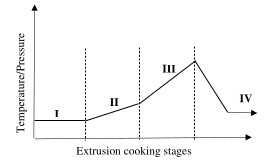
\includegraphics{115}
		    \caption*{}
		\label{fig:Q115}
	\end{figure}
    \begin{enumerate}
        \item I- Feeding, II - Cooking, III - Kneading, IV - Expansion
        \item I- Kneading, II - Feeding, III - Cooking, IV - Expansion
        \item I- Feeding, II - Kneading, III - Cooking, IV - Expansion
        \item I- Cooking, II - Kneading, III - Feeding, IV - Expansion
    \end{enumerate}

    \item \begin{minipage}{0.45\textwidth}
    Match the method/value used for measuring lipid characteristics in Group I with the corresponding properties indicated by them, in Group II.
    \begin{itemize}
        \item[P.] Thiobarbituric acid test
        \item[Q.] Rancimat method
        \item[R.] Peroxide value
        \item[S.] Iodine value
    \end{itemize}
    \end{minipage}
    \begin{minipage}{0.45\textwidth}
    \begin{itemize}
        \item[1.] Induction time
        \item[2.] Degree of unsaturation
        \item[3.] Carbonyl content
        \item[4.] Hydroperoxide content
    \end{itemize}
    \end{minipage}
    \begin{enumerate}
        \item P-3, Q-1, R-4, S-2
        \item P-1, Q-3, R-4, S-2
        \item P-3, Q-1, R-2, S-4
        \item P-3, Q-4, R-1, S-2
    \end{enumerate}

    \item \begin{minipage}{0.45\textwidth}
    Match the peeling technique in Group I with the vegetable, for which it is used in industry, given in Group II.
    \begin{itemize}
        \item[P.] Knife peeling
        \item[Q.] Abrasion peeling
        \item[R.] Flame peeling
        \item[S.] Flash peeling
    \end{itemize}
    \end{minipage}
    \begin{minipage}{0.45\textwidth}
    \begin{itemize}
        \item[1.] Brinjal
        \item[2.] Tomato
        \item[3.] Potato
        \item[4.] Cucumber
    \end{itemize}
    \end{minipage}
    \begin{enumerate}
        \item P-3, Q-4, R-1, S-2
        \item P-4, Q-1, R-3, S-2
        \item P-4, Q-3, R-2, S-1
        \item P-4, Q-3, R-1, S-2
    \end{enumerate}

    \item \begin{minipage}{0.45\textwidth}
    Match the process in Group I with the related food component in Group II.
    \begin{itemize}
        \item[P.] Caramelization
        \item[Q.] Denaturation
        \item[R.] Oxidation
        \item[S.] Bleaching
    \end{itemize}
    \end{minipage}
    \begin{minipage}{0.45\textwidth}
    \begin{itemize}
        \item[1.] Lipid
        \item[2.] Sugar
        \item[3.] Pigment
        \item[4.] Enzyme
    \end{itemize}
    \end{minipage}
    \begin{enumerate}
        \item P-2, Q-4, R-1, S-3
        \item P-2, Q-1, R-4, S-3
        \item P-1, Q-3, R-2, S-4
        \item P-2, Q-1, R-3, S-4
    \end{enumerate}

    \item Identify the correct statement(s) related to grain polysaccharides among the followings.
    \begin{enumerate}
        \item Dextrin are a group of low molecular weight polysaccharides produced by dry hydrolysis of starch.
        \item Amylose is a linear polymer of D-glucose units joined by alpha (1-4) glycoside linkages.
        \item Amylopectin is a branched chain polymer of D-galactose monomer units.
        \item Retrogradation is a process of reassociation of amylose and formation of crystalline structure by gelatinized starch upon cooling.
    \end{enumerate}

    \item A sample of glucose isomerase enzyme converts 15 moles of substrate glucose into product fructose min$^-1$ mL$^-1$ under standard assay conditions. The enzyme activity of the glucose isomerase in International Unit (IU) is \rule{1 cm}{0.15 mm} (in integer).

    \item If D10 for Salmonella in egg yolk is 0.75 kGy, calculate the radiation dose in kGy (rounded off to 2 decimal places) required for reducing the Salmonella count in egg yolk by 8 log cycles.

    \item The average moisture binding energy of a textured protein product (TPP) at 8\% moisture content (dry basis) is 3200 cal.mol$^{-1}$. If the water activity of the TPP at the above moisture content is 0.30 at 30 $\celsius$C, the water activity of the sample at 45 $\celsius$C is \rule{1 cm}{0.15 mm} (rounded off to 2 decimal places). The value of Gas constant R= 1.987 cal.mol$^{-1}$.$K{^-1}$.
\end{enumerate}

\end{document}
